\section{Methodology}
For this tree detection task we implemented a U-Net regression architecture with a temporal attention mask which predicts the number of trees per pixel of Sentinel-2 data where the prediction labels are derived from communal tree cadasters. 
\subsection{Data Processing}

The first methodological step was fetching the different datasets on Sentinel-2 images, tree locations and OSM information.

\begin{figure}[H] 
    \centering
    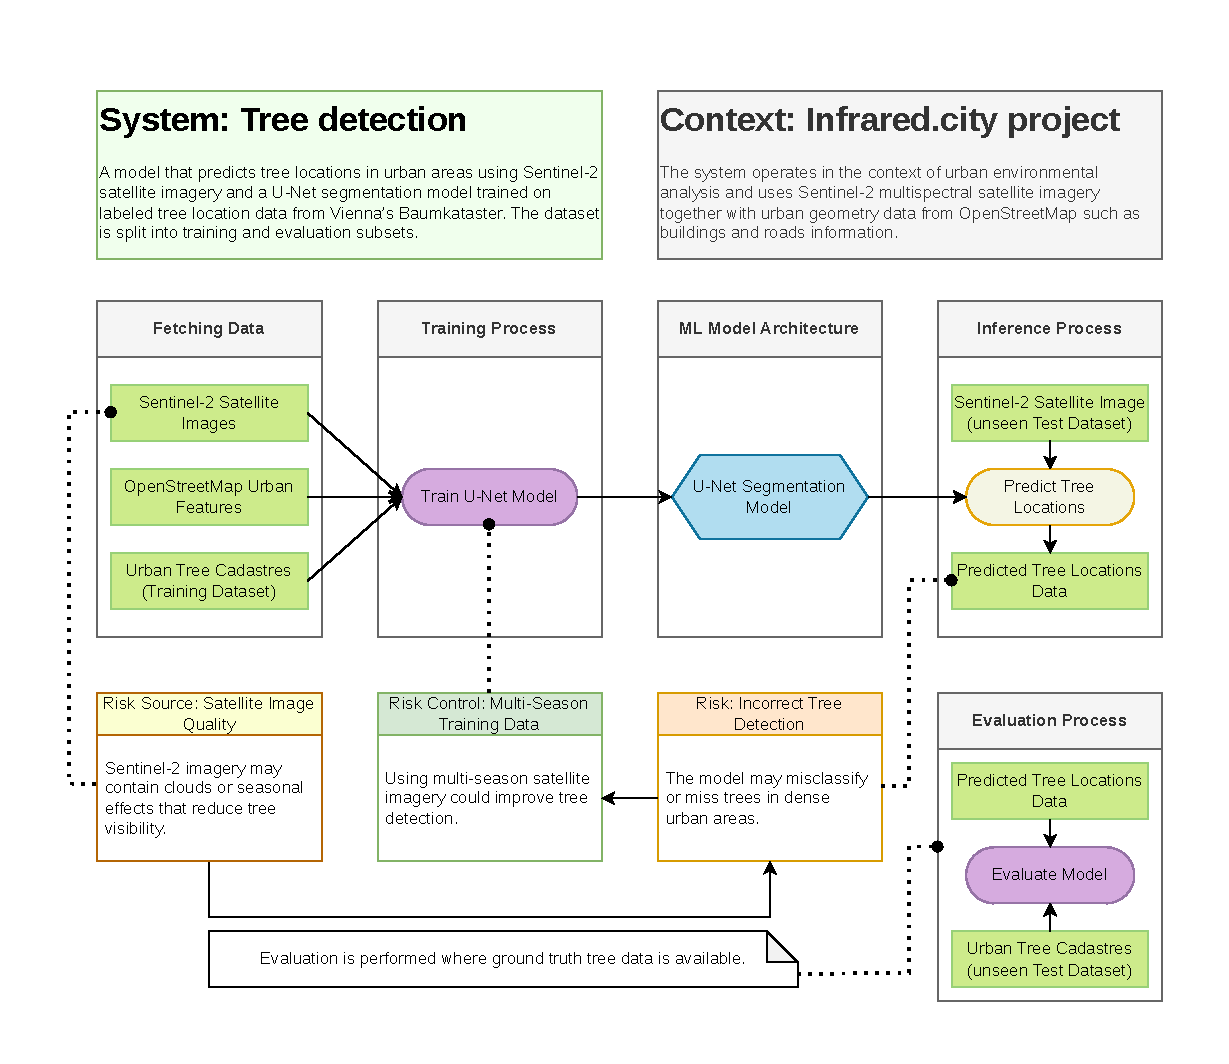
\includegraphics[width=\textwidth]{images/refined_beam_treeDetection_infraredCity.drawio.pdf}
    \caption{BEAM model of the proposed tree detection system.}
    \label{fig:overview_beam}
\end{figure}

\subsection{Data Preprocessing for ML}
Through our EDA and some manual checking we were able to find some important properties about our data which influence the needed preprocessing pipeline and the model architecture. The most important aspects were that only around 4% of pixels contained trees in the ground truth and that most trees on private property were missing in our ground truth. 
\\
The first step in our preprocessing pipeline for the machine learning part of our process was to split the Sentinel-2 images into smaller patches which were easier to load into memory and to process for our model. To end up with more patches we also implemented stride, so patches were overlapping. 
\\
We then aligned the ground truth from the tree cadasters with the Sentinel-2 patches, labeled each patch with the corresponding month when the image was taken and normalized the values so it would be easier for the model to learn their patterns. As the data was already very sparse, we decided to drop patches with a low number of trees.
\\
By manual checking we noticed that there was a significant number of trees missing in our ground truth which is due to the fact that trees on private property are not registered in the public tree cadasters. Our first attempt to solve this problem was to get data on what is private property, but this was more tedious than we expected because there is no complete available data on what is private property for any city. 
\\
We then noticed that the ground truth was normally very clustered, meaning that normally pixels containing trees in the ground truth were closer together and there were significant holes between them with many pixels containing zero trees. Which makes sense as private and public areas also are somewhat clustered. So, we switched to an approach where we would only use pixels for training where there were trees in a specified radius to avoid training on those large private areas falsely containing zero trees in the ground truth. Similar approaches already delivered promising results in former projects \cite{lin2016scribblesup}.
\subsection{Model}
Former papers suggest that for image segmentation using satellite data the U-Net deep learning model is the most accurate for detecting objects, for example street detection \cite{pesek2024convolution} as well as crop field detection \cite{garnot2021panoptic}. Furthermore, last year's \textit{infrared.city} project also tried implementing a U-Net architecture but failed to yield promising results, also the data coaches deem it a well-fitting model.
\\
The U-Net model is a special type of Convolutional Neural Network and consists of a contracting path and an expanding path.
\\
First, the satellite image is put through an input convolution, so it has the correct structure for further processing. It is then passed into the contracting path to down-sample the data in the convolution and pooling layers, which are used to extract features from the original imagery. Our model uses four convolutional layers where during contraction for each layer the image size gets smaller due to pooling meanwhile evermore features are extracted from the images. The same process happens vice versa for the expansionary path.  The expanding path consists of the same structure of convolution and pooling layers but this time used to up-sample the before contracted imagery \cite{aramendia2024}. 
\\
As suggested in similar work this project will use skip connections between the expanding and contracting path as well as a temporal attention algorithm with multi-head attention to prioritize more meaningful images from the three months \cite{garnot2021panoptic} and take advantage of the seasonality and changing vegetation of trees.
\\
The outputs of the up-sampling block are then going through two separate final convolutional blocks where one head is supposed to predict the probability of a pixel containing any trees and the other head outputs the number of trees for each pixel. The two results are then multiplied to get the final prediction. This method helps overcome the problem that most pixels in the ground truth contain no trees and the issue that the labels are incomplete by enabling the model to learn uncertainty about presence in the probability head and about the abundance of trees in areas where they likely exist in the count head. The multiplication process suppresses false positive counts in areas with obviously no trees \cite{sileshi2009traditional} \cite{caruana1997multitask}.
\\
During the training process the results of the probability head together with the ground truth are put through a weighted binary cross-entropy loss as we want results between 0 and 1 \cite{bishop2006prml}. The results of the count head are first log transformed to ensure that outliers do not have too much of an impact on the gradients, then smooth L1 loss was used due to its robustness to labeling errors \cite{huber1964robust}. 
\\
Figure~\ref{fig:beam} presents the BEAM representation of the proposed tree detection model

\begin{figure}[H] 
    \centering
    
\includegraphics[width=\textwidth]{images/U-Net.png}
    \caption{BEAM model of the proposed tree detection model}
\end{figure}